
\chapter[Related Works]{Related Works}
\graphicspath{ {images/stateOfArt} }

\section{The second, math section}
Wettel in his thesis \cite{Wettel2011}, defined a city metaphor for software visualization that represents software as cities. His work represents packages as districts and classes as buildings. This metaphor was applied in different contexts related to reverse engineering (program comprehension, software evolution, software quality) to demonstrate metaphor's versatility. As a result, he found evidence that his approach works. However, he claims that city metaphor brings visual and layout limitations (not all visualization techniques fit well with it). Under those circumstances, he preferred simplicity over the accuracy, so he obtained a simple visual language that facilitates comprehension of data. 
He conducted an experiment of the evidence that the city metaphor enables the creation of efficient software visualizations. His approach was implemented by a software visualization tool called CodeCity that supports the city metaphor. 

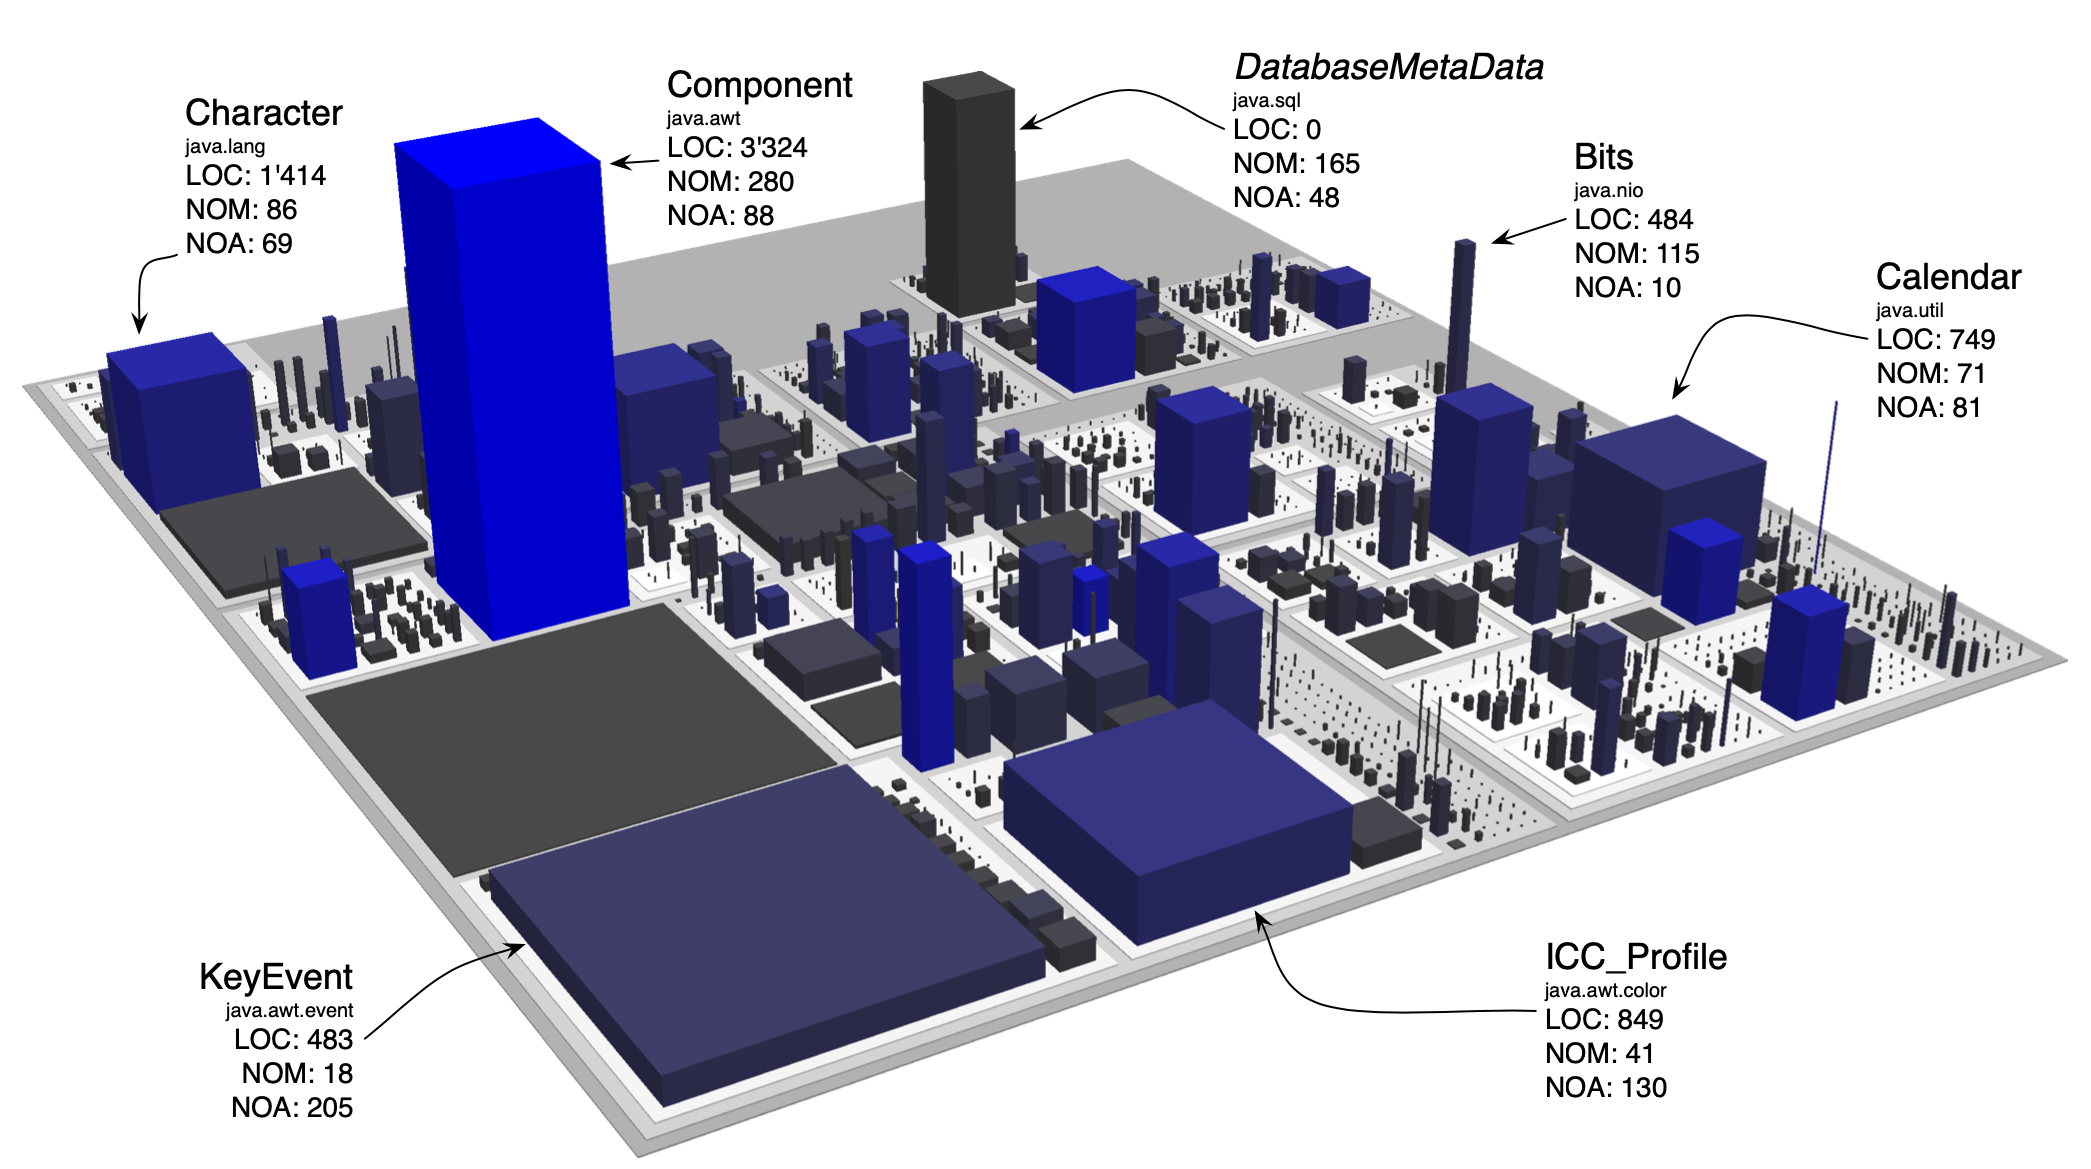
\includegraphics[width=\textwidth]{CodeCity.png}